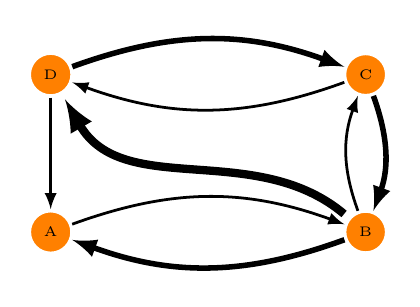
\begin{tikzpicture}[font=\tiny]
    \tikzstyle{node_style} = [draw=white, very thick, circle, fill=orange]
    \tikzstyle{arrow_style1} = [->, black, line width=1, >=latex]
    \tikzstyle{arrow_style2} = [->, black, line width=2, >=latex]
    \tikzstyle{arrow_style3} = [->, black, line width=3, >=latex]
    \tikzstyle{edge_style2} = [lightgray, line width=1]


    \node[node_style] (n1) at (0,0) {A};
    \node[node_style] (n2) at (4,0) {B};
    \node[node_style] (n3) at (4,2) {C};
    \node[node_style] (n4) at (0,2) {D};

    \draw[arrow_style1] (n1) edge [bend left=20] (n2);
    \draw[arrow_style2] (n2) edge [bend left=20] (n1);
    \draw[arrow_style1] (n2) edge [bend left=20] (n3);
    \draw[arrow_style2] (n3) edge [bend left=20] (n2);
    \draw[arrow_style1] (n3) edge [bend left=20] (n4);
    \draw[arrow_style2] (n4) edge [bend left=20] (n3);
    \draw[arrow_style1] (n4) edge (n1);
    \draw[arrow_style3, shorten <=2pt, shorten >=2pt] (n2) edge [out=140, in=-60] (n4);
\end{tikzpicture}
